\documentclass[paper=a4,parskip=half,DIV=12]{leetcode}

\usepackage[T1]{fontenc}
\usepackage[utf8]{inputenc}
\usepackage{courier}
\usepackage{tgtermes,newtxtext,newtxmath}
\usepackage[pdftex,colorlinks,allcolors=blue]{hyperref}
\usepackage{natbib}

\usepackage{amsmath,amsfonts}
\usepackage{tikz}
\usetikzlibrary{arrows,calc,graphs,matrix,quotes}

\setcitestyle{numbers,square,comma}

\begin{document}

\serietitle{LeetCode contests solutions}
\title{1601. Maximum Number of Achievable Transfer Requests~\cite{leetcode:1601}}
\subtitle{}
\author{Paweł Tomulik}
\date{2024-06-20}
\maketitle

\section{Description}
\label{sec:description}

We have $N$ buildings numbered from $0$ to $N - 1$. Each building has a~number
of employees. It's transfer season, and some employees want to change the
building they reside in.

You are given an array \texttt{requests} where \texttt{requests[i] = [from$_i$,
to$_i$]} represents an employee's request to transfer from building
\texttt{from$_i$} to building \texttt{to$_i$}.

All buildings are full, so a list of requests is achievable only if for each
building, the net change in employee transfers is zero. This means the number
of employees leaving is equal to the number of employees moving in. For example
if $N = 3$ and two employees are leaving building $0$, one is leaving building
$1$, and one is leaving building $2$, there should be two employees moving to
building $0$, one employee moving to building $1$, and one employee moving to
building $2$.

Return the \textbf{maximum number of achievable requests}.

\section{Solution}
\label{sec:solution}

\subsection{Complexity}
\label{sec:complexity}

\subsection{Solution description}
\label{sec:solution-description}

This problem can be modelled with a~directed multi-graph. Graph nodes represent
buildings, edges correspond to transfer requests. Instead of drawing multiple
edges connecting a~single pair $i,j$ of vertices, we'll just draw a~single arc
and assign it an integer $r_{ij}$ to represent multiplicity:
%%%%%%%%%%%%%%%%%%%%%%%%%%%%%%%%%%%%%%%%%%%%%%%%%%%%%%%%%%%%%%%%%%%%%%%%%%%%%
\begin{equation}
    r_{ij} \in \mathbb{N}, \; i, j \in \{ 0, 1, \dots N-1 \}.
    \label{eq:49EZ8}
\end{equation}
%%%%%%%%%%%%%%%%%%%%%%%%%%%%%%%%%%%%%%%%%%%%%%%%%%%%%%%%%%%%%%%%%%%%%%%%%%%%%

Balanced transfers are realized along cycles on the graph. Simplest possible
case is a~request to stay in same building -- a~{\em loop} on the graph.
Next example is a pair of nodes~${(i, j)}$ forming a cycle $i \to j \to i$
(figure~\ref{fig:DRV1T}). The maximum number $t_{ij}$ of possible transfers
between buildings $i$ and $j$ is in this case
%%%%%%%%%%%%%%%%%%%%%%%%%%%%%%%%%%%%%%%%%%%%%%%%%%%%%%%%%%%%%%%%%%%%%%%%%%%%%
\begin{equation}
  t_{ij} = 2 r_{\min} = 2 \min{(r_{ij}, r_{ji})}.
  \label{eq:FMMLO}
\end{equation}
%%%%%%%%%%%%%%%%%%%%%%%%%%%%%%%%%%%%%%%%%%%%%%%%%%%%%%%%%%%%%%%%%%%%%%%%%%%%%
%%%%%%%%%%%%%%%%%%%%%%%%%%%%%%%%%%%%%%%%%%%%%%%%%%%%%%%%%%%%%%%%%%%%%%%%%%%%%
\begin{figure}[htbp]
  \centering
  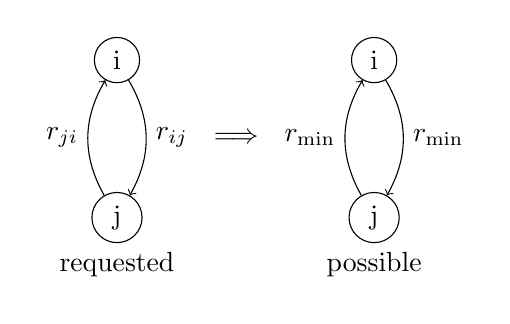
\begin{tikzpicture}
    \matrix {
      \graph[nodes={draw,circle}, clockwise=2] {
        i; j;
        i -> [bend left, "$r_{ij}$"] j ->[bend left,"$r_{ji}$"] i;
      }; & \node {$\implies$}; & \graph[nodes={draw,circle}, clockwise=2] {
        i; j;
        i -> [bend left, "$r_{\min}$"] j ->[bend left,"$r_{\min}$"] i;
      }; \\
      \node {requested}; & & \node {possible}; \\
    };
  \end{tikzpicture}
  \caption{Example two-node cycle. The number of requests from $i$ to $j$ is
  $r_{ij}$, from $j$ to $i$ is $r_{ji}$. The maximum possible number of mutual
  transfers depends on the $r_{\min} = \min{(r_{ij}, r_{ji})}$.}
  \label{fig:DRV1T}
\end{figure}
%%%%%%%%%%%%%%%%%%%%%%%%%%%%%%%%%%%%%%%%%%%%%%%%%%%%%%%%%%%%%%%%%%%%%%%%%%%%%
Note, that if we remove all the edges that comprise the cycle, still some edges
may be left on the graph (rejected requests). In this case, the number of
rejected requests is $r_{ij} + r_{ji} - 2 r_{\min}$. Finding the number of
achievable transfers is equivalent to finding the minimum number of requests
that must be rejected.

For a~three-node/three-edge cycle, as in figure~\ref{fig:U5GUM}, the maximum
possible number of transfers is
%%%%%%%%%%%%%%%%%%%%%%%%%%%%%%%%%%%%%%%%%%%%%%%%%%%%%%%%%%%%%%%%%%%%%%%%%%%%%
\begin{equation}
  t_{ijk} = 3 r_{\min} = 3 \min{(r_{ij}, r_{jk}, r_{ki})}
 \label{eq:S95QR}
\end{equation}
%%%%%%%%%%%%%%%%%%%%%%%%%%%%%%%%%%%%%%%%%%%%%%%%%%%%%%%%%%%%%%%%%%%%%%%%%%%%%
%%%%%%%%%%%%%%%%%%%%%%%%%%%%%%%%%%%%%%%%%%%%%%%%%%%%%%%%%%%%%%%%%%%%%%%%%%%%%
\begin{figure}[htbp]
  \centering
  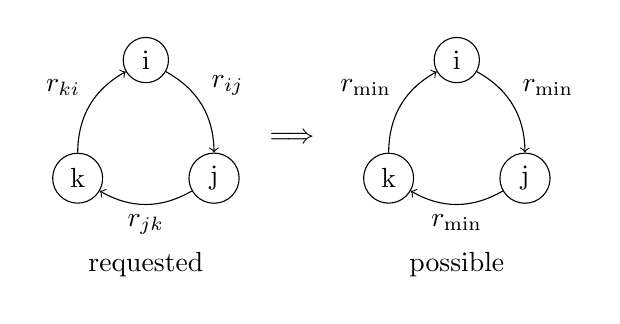
\begin{tikzpicture}
    \matrix {
      \graph[nodes={draw,circle}, clockwise=3] {
        i; j; k;
        i ->[bend left, "$r_{ij}$"] j ->[bend left,"$r_{jk}$"]  k ->[bend left, "$r_{ki}$"] i;
      }; & \node {$\implies$}; & \graph[nodes={draw,circle}, clockwise=3] {
        i; j; k;
        i ->[bend left, "$r_{\min}$"] j ->[bend left,"$r_{\min}$"]  k ->[bend left, "$r_{\min}$"] i;
      }; \\
      \node {requested}; & & \node {possible}; \\
    };
  \end{tikzpicture}
  \caption{Example three-node cycle}
  \label{fig:U5GUM}
\end{figure}
%%%%%%%%%%%%%%%%%%%%%%%%%%%%%%%%%%%%%%%%%%%%%%%%%%%%%%%%%%%%%%%%%%%%%%%%%%%%%

In general, the~number of possible transfers along an~isolated
$K$-node/$K$-edge cycle is a~multiple of~$K$, and has the form
$t = K r_{\min}$, where $r_{\min}$ is the minimum weight along the path.

%%We guess, that for a~$K$-node cycle $\mathcal{C}$, the maximum possible number
%%of transfers is
%%%%%%%%%%%%%%%%%%%%%%%%%%%%%%%%%%%%%%%%%%%%%%%%%%%%%%%%%%%%%%%%%%%%%%%%%%%%%%%
%%\begin{equation}
%%  m_{\mathcal{C}} = K \min_{e_{ij} \in \mathcal{C}}{\{e_{ij}\}}
%%  \label{eq:63VA3}
%%\end{equation}
%%%%%%%%%%%%%%%%%%%%%%%%%%%%%%%%%%%%%%%%%%%%%%%%%%%%%%%%%%%%%%%%%%%%%%%%%%%%%%%

Isolated cycles are simple. In reality, however, cycles can partially overlap.
Consider a~three node graph with two different cycles as shown on
figure~\ref{fig:XDUOL}. Total number of requests is $r_{ij} + r_{jk} + r_{ki} +
r_{kj}$, but there are constraints limiting the possible number of transfers.
%%%%%%%%%%%%%%%%%%%%%%%%%%%%%%%%%%%%%%%%%%%%%%%%%%%%%%%%%%%%%%%%%%%%%%%%%%%%%
\begin{figure}[htbp]
  \centering
  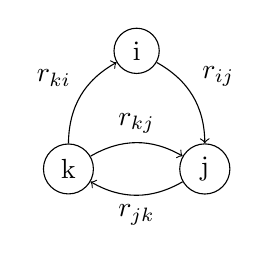
\begin{tikzpicture}
    \graph[nodes={draw,circle}, clockwise=3]{
      i; j; k;
      i ->[bend left, "$r_{ij}$"] j
        ->[bend left, "$r_{jk}$"] k
        ->[bend left, "$r_{ki}$"] i;
      k ->[bend left, "$r_{kj}$"] j;
    };
  \end{tikzpicture}
  \caption{Example three-node graph with two cycles}
  \label{fig:XDUOL}
\end{figure}
%%%%%%%%%%%%%%%%%%%%%%%%%%%%%%%%%%%%%%%%%%%%%%%%%%%%%%%%%%%%%%%%%%%%%%%%%%%%%
The edge $j \to k$ is shared between cycles $i \to j \to k \to i$ and $j \to k
\to j$. From the other perspective, the edge $j \to k$ contributes to either
the $i \to j \to k \to i$ or $j \to k \to j$, or to both.

\bibliographystyle{unsrtnat}
\bibliography{leetcode}

\end{document}

%\label{??:63VA3}
%\label{??:W6D11}
%\label{??:SJ2HQ}
%\label{??:0NZPS}
%\label{??:A20W8}
%\label{??:6M1IM}
%\label{??:KSU4J}
%\label{??:KRXUE}
%\label{??:P2GTP}
%\label{??:I4AB9}
%\label{??:D2Y3O}
%\label{??:XW7AC}
%\label{??:6NYTI}
%\label{??:57L58}
%\label{??:HP3C4}
%\label{??:UDSSB}
%\label{??:YA13L}
%\label{??:4B7KI}

% vim: set syntax=tex tabstop=2 shiftwidth=2 expandtab spell spelllang=en:
